\twocolumn\newpage\thispagestyle{empty}
\chapter[靛蓝的红枫 \~{} Crystal Maple]{
\begin{center}
    {\Large \textbf{靛蓝的红枫 \~{} Crystal Maple——Maple与幻想乡的二三事}}\\
    {\normalsize\itshapeCJK 小麻雀}\vspace*{2em}
\end{center}}
\addauthor{小麻雀}
\parindent = 0pt

    {\bfseries \large 某年某月某日晚上,妖怪兽道,夜雀食堂}

【人物:老板娘米斯琪,主人公橙,顾客萃香等,解说射命丸文】

\textbf{橙}\textit{(激动状)}:老板娘,来一瓶啤酒、一份秘制小鱼干!

\textbf{米斯琪}:本店不向未成年妖怪——咦,这不是橙吗?

\textbf{萃香}:橙,听说你上大学了?恭喜呀,大学生活一定很有趣吧。

\textbf{橙}\textit{(略微泄气)}:呜哇别提了,大学里一点也不好玩。蓝大人给的作业
又多又难,数学也不会,物理也不会,写一会儿就想摸鱼了……

\textbf{米斯琪}\textit{(思索状)}:所以来这里也是?

\textbf{橙}:千万别告诉蓝大人!\textit{(慌乱状)}咱是偷偷溜出来的,要是被蓝大
人发现的话,不死也得掉层皮!

\textbf{米斯琪}:蓝有那么可怕么。\textit{(米斯琪流汗状)}话说回来你的
作业怎么办,总不能拿摸鱼去交差吧。

\textbf{橙}\textit{(流汗状)}:这个嘛……

\begin{figure}[htpb]
    \centering
    \line(1,0){7.5cm}\\

\end{figure}
以下是橙内心活动:

{\CJKfontspec{FandolFang-Regular.otf}  蓝(微笑状):橙,作业做得怎么样了呀?

橙(心虚):好的。

蓝:好什么好?我看看,嗯?(蓝笑容逐渐凝固)橙你过来来。

橙(瑟瑟发抖):好的。}

\begin{center}
    \textbf{\large 四面楚歌?!八雲藍能否一擊必殺?\\ 次回:橙喵之死!}
\end{center}

\begin{figure}[htpb]
    \centering
    \line(1,0){7.5cm}\\

\end{figure}

\textbf{橙}:不对不对,妖贵有自知之明,可是咱真的不会呀。\textit{(橙瘫在餐台上大哭状)}

\textbf{米斯琪}:对了,前阵子妖怪之山的人来了之后留下了这个东西。(\textit{米斯琪转身走进库房,片刻后)}锵锵,就是这个。

\textbf{橙}:这是,一台电脑?

\textbf{米斯琪}:其他人似乎是这么叫的,他们想在幻想乡搞什么互联网,于是就送了我一台,现在用在店里记账,我这鸟脑袋是用不明白。只能都交给响子了。

\textbf{橙}:话说回来响子呢?

萃香:是啊是啊老板娘,从刚才我进来到现在也没见到响子。

\textbf{米斯琪}:响子的话在睡觉啦。\textit{(阿嚏~巨大的喷嚏声从幕后传来)}真是的,又不好好盖被子,秋天来了这样子会感冒的,我去去就来哦。\textit{(米斯琪退场,射命丸文走进)}

\textbf{射命丸文}:哦呀哦呀,这不是橙吗,偷偷跑出来了?小心我明天登在
报纸上哦~(看向电脑,迟疑)啊,这不是我们天狗和河童一起开发的
电脑吗。

\textbf{橙}:原来是你们做出来的呀,不过有什么用呢?

\textbf{射命丸文}:\textit{(走近电脑拿起鼠标)}具体的话我也不是很清楚,不过我
知道这个软件是我们开发的。
\begin{figure}[h]
    \centering
    
\includegraphics[scale=1]{logo.PNG}
\end{figure}
前阵子果果还和甲方吵得不可开交呢,点开看看?

\begin{figure}[h]
    \centering
    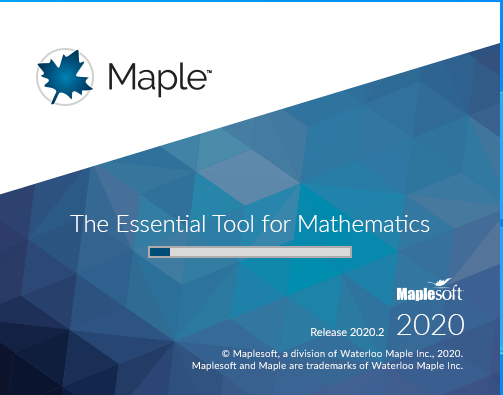
\includegraphics[scale=0.3]{start.PNG}
\end{figure}

\begin{figure}[h]
    \centering
    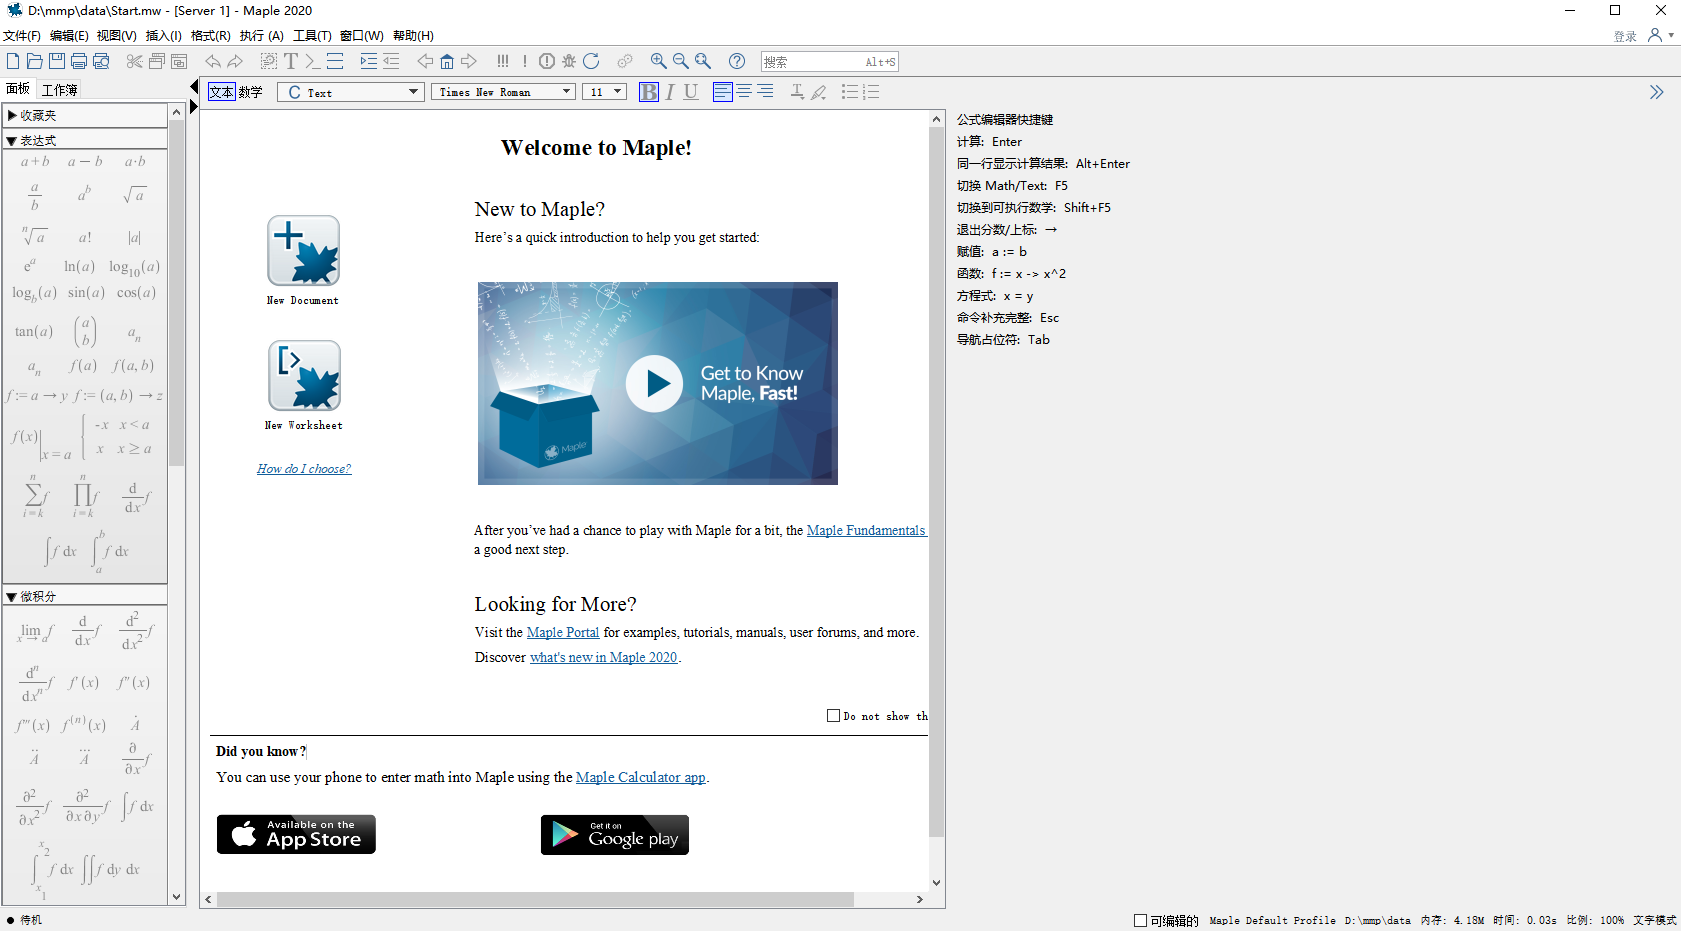
\includegraphics[scale=0.16]{homepage.PNG}
\end{figure}

\textbf{橙}:好,好复杂,还有好多看不懂的文字。\textit{(橙眼睛里黑线绕圈圈)}

射命丸文\textit{(目不转睛盯着屏幕)}:也就是看起来复杂而已,你听我讲讲就明白了。这个软件叫Maple ,英文里是枫叶的意思,是果果的品味哦。妖怪之山的数学家和工程师为了方便数学的计算和工程应用的模拟,一起开发了这个软件。最上面的是菜单栏,等会儿再讲,我们先新建一个项目。

\textbf{橙}\textit{(发呆状)}:可是这里有两个选项哎。

\textbf{射命丸文}:刚接触Maple的话,只需要用下面的工作表模式就行了,先把它点开。

\begin{center}
    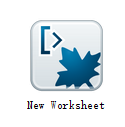
\includegraphics[scale=1]{worksheetlogo.PNG}
\end{center}

\begin{figure}[h]
    \centering
    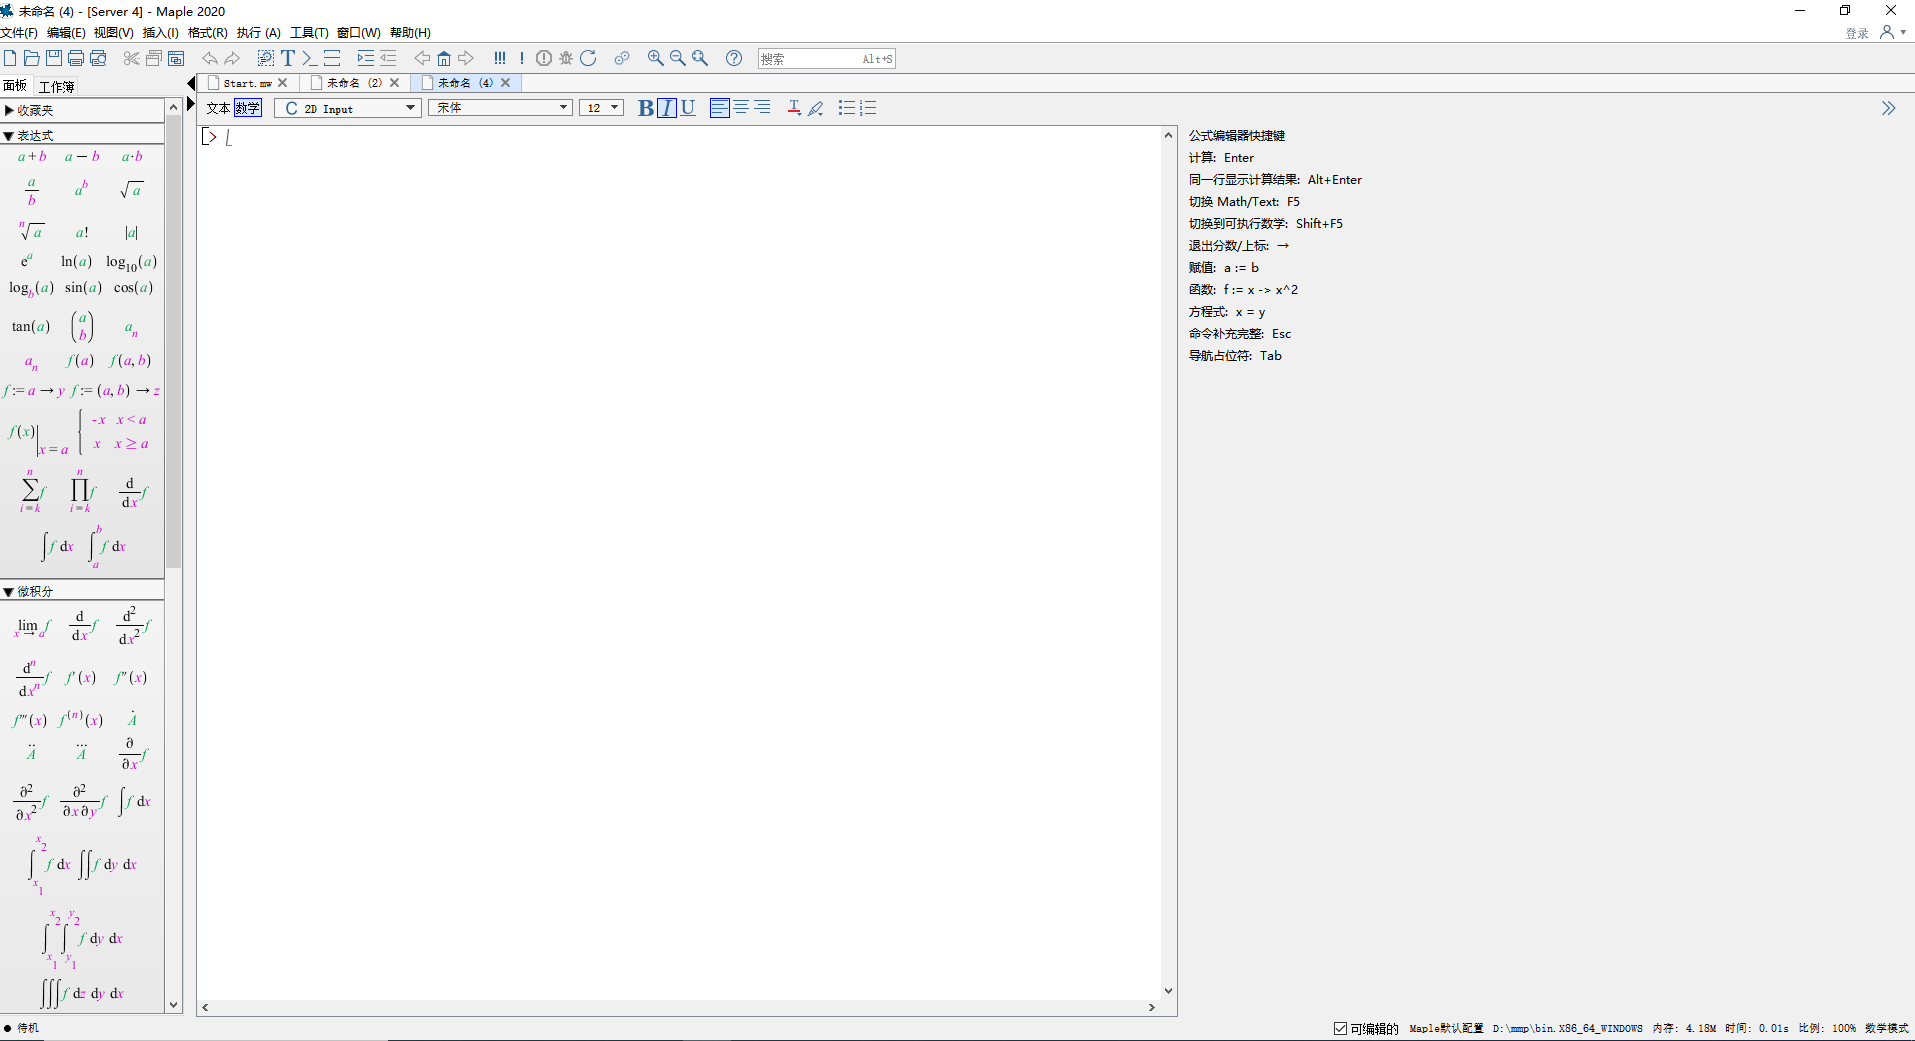
\includegraphics[width=8cm]{worksheet.PNG}
\end{figure}

Maple 的受众很广,像橙这样的大学生,或是像蓝那样的数学 家,又或者是像荷取那样的工程师,都可以是Maple的用户。橙你有什 么不会的题吗?

\textbf{橙}\textit{(眼睛放光状)}:有的有的,这个题我就不会!
\begin{figure}[htpb]
    \centering
    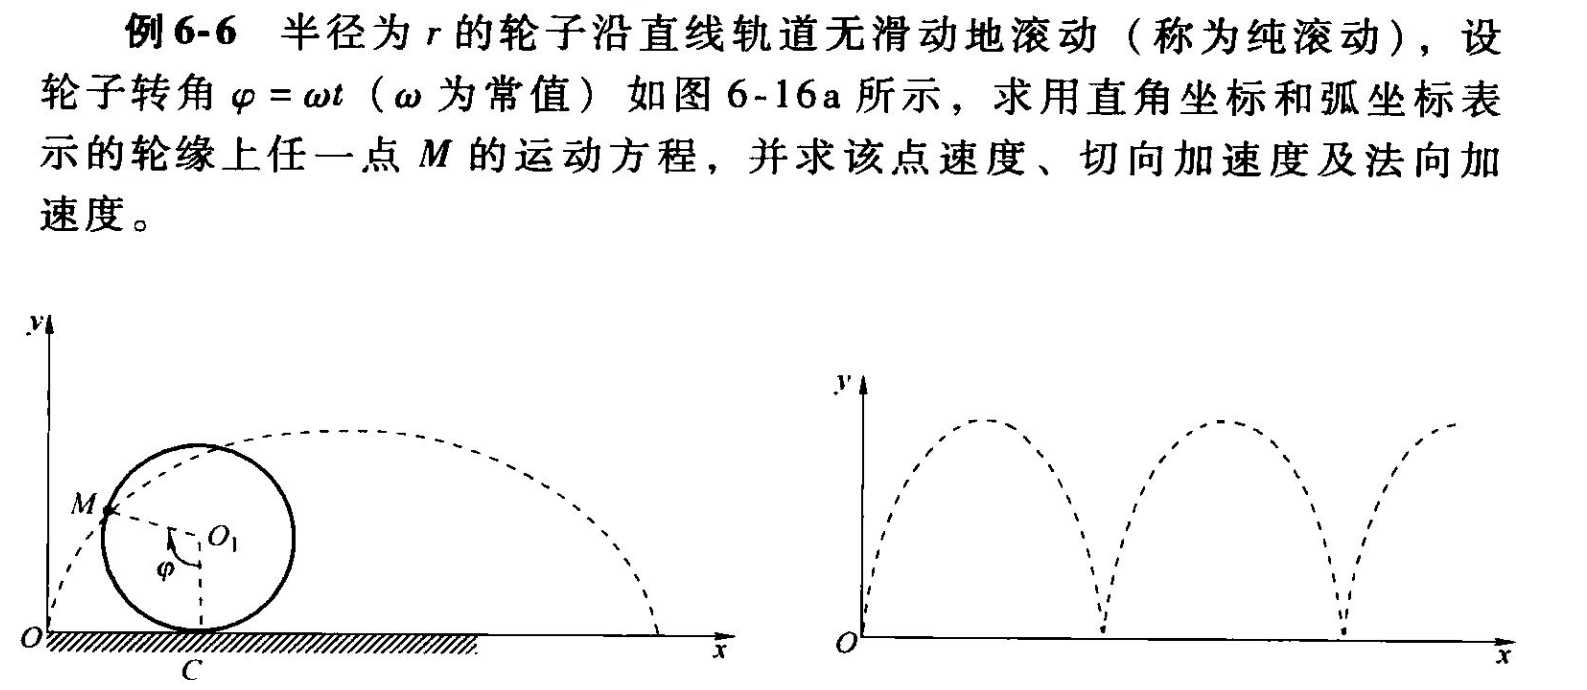
\includegraphics[width=8cm]{phy.PNG}
\end{figure}

\textbf{射命丸文}\textit{(依旧目不转睛)}:那就拿这个场景举例子吧,看
我打出的代码。

\begin{figure}[h]
    \centering
    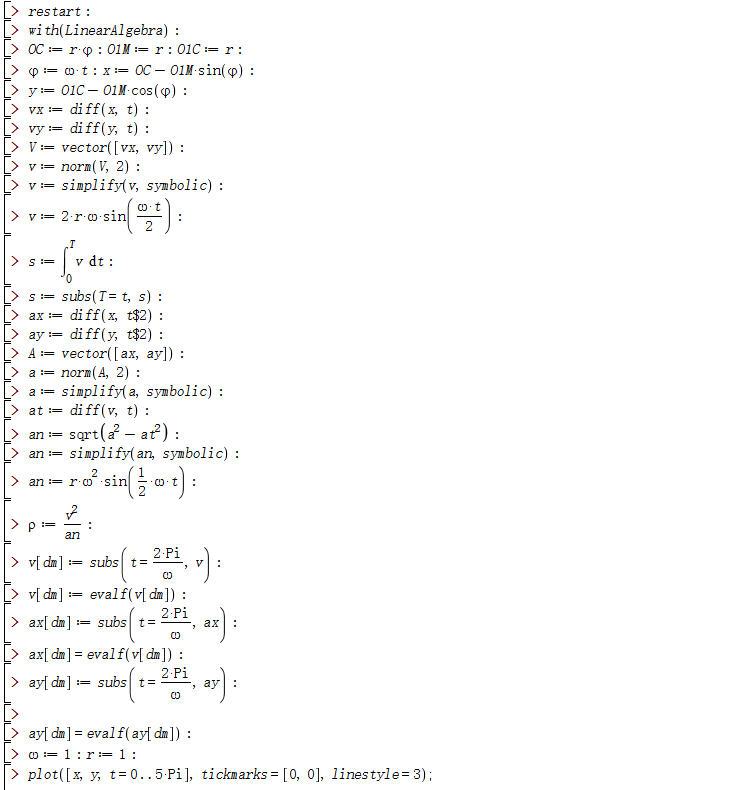
\includegraphics[width=12cm]{non;.PNG}
\end{figure}

\textbf{橙}\textit{(后仰)}:不愧是天狗,打字速度好快!

\textbf{射命丸文}\textit{(得意状)}:Maple是交互式编程,支持符号运算,你可以一
边运算一边化简你的表达式,如果你不想这样每一行都出现结果,可
以在每一行的结束加上一个“\verb":"”,这样的话代码看起来就会清爽很多。

\begin{center}
    \includegraphics[width=16cm]{with:.PNG}
\end{center}

左侧可以直观地看出每一个变量当前的符号表达式,这对于物理以及工程上的计算十分重要。

\begin{center}
    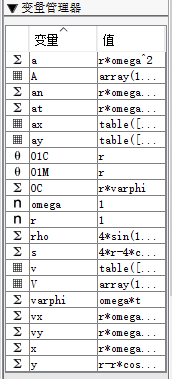
\includegraphics[width=3cm]{variable manager.PNG}
\end{center}

\textbf{橙}\textit{(勉为其难状)}:但是,咱好像不会微积分呢!

\textbf{射命丸文}\textit{(猛然转过头、石化震惊状)}:哈?

\textbf{橙}\textit{(跪下磕头)}:求求姑奶奶救救咱,咱不想被蓝大人杀害哇啊!!!!!!

\textbf{射命丸文}\textit{(傲娇脸)}:哼,那我就勉为其难教教你吧。你打开这个
MathApp,这里面是一些闲得胃疼的数学家整合的数学应用,各种
用途的都有,建议你上手之后自己点开看一下,就当玩玩儿。

\begin{figure}[h]
    \centering
    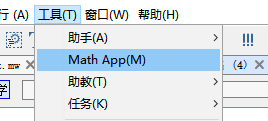
\includegraphics[scale=1]{MathApp.PNG}
\end{figure}
\begin{figure}[h]
    \centering
    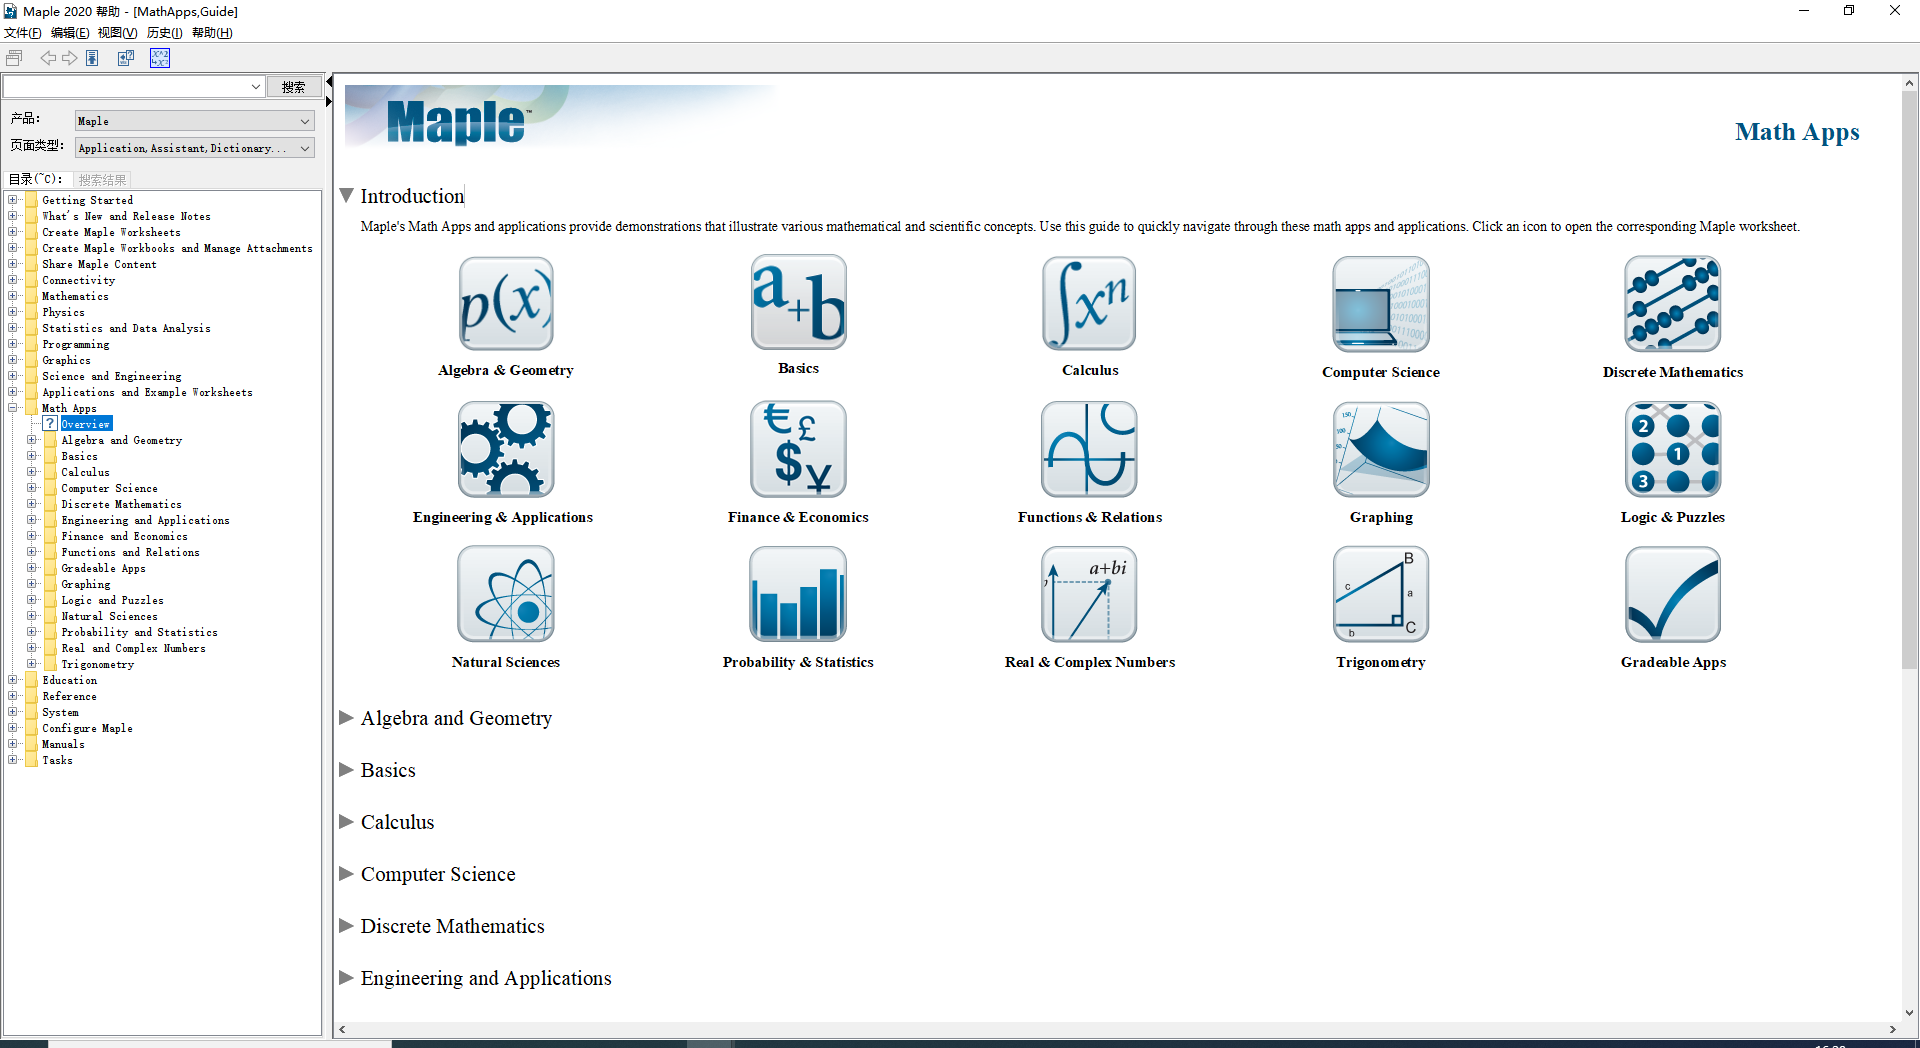
\includegraphics[width=8cm]{Apps.PNG}
\end{figure}

Calculus\footnote{编者注:即上图中的$\int
        x^n$.}里面有给你们理解微积分准备的小程序,比如这个程序,就可以很直观地感受到球的体积的来历。

\begin{figure}[htpb]
    \centering
    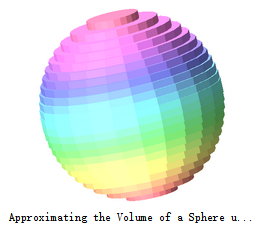
\includegraphics[scale=0.2]{sphere.PNG}
\end{figure}

除此之外,还有一套集成的数学计算工具,在MathApp下面的助教选项里。
\begin{figure}[htpb]
    \centering
    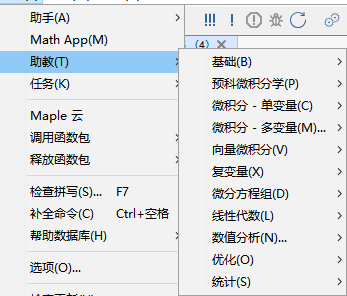
\includegraphics[width=7cm]{助教.PNG}
\end{figure}

\textbf{橙}\textit{(苦笑状)}:虽然Maple虽然功能很强大,但是咱还是做不出蓝大人给的题喵。

\textbf{射命丸文}\textit{(弯腰严肃地指着橙说)}:当然啦!学习只有自己学,不要想着走捷径,否则
你偷的懒以后会自己找上门来的哦。

\textbf{橙}\textit{(耷拉着耳朵状)}:咱知道了喵。咱不摸鱼了,一定好好学习。

\textit{(米斯琪回到舞台)}

\textbf{米斯琪}\textit{(银铃般的笑声)}:橙的大学生活才刚开始,不要想着有捷径可以走哦。

\textbf{橙}\textit{(快要哭了)}:上大学真的有用吗?咱也好羡慕老板娘,明明没有上过大学却
经营着这样一家体面的夜雀食堂,幻想乡的大家也都发自内心地喜欢着老板娘。

\textbf{米斯琪}\textit{(从后面温柔地抱住橙)}
:不是的哦,老板娘我呀,也不是一开始就有这样
一家店的,而是一点点积累经验
、品尝过一次次失败的滋味、和幻想乡的大家一起
走到现在的。老板娘因为没文化吃过亏,不希望橙以后也遇到同样的事情。

\textbf{橙}\textit{(大哭)}:咱知道了喵,谢谢老板娘,也谢谢文文。\textit{(文文竖大拇指)(
    约半分钟后橙擦干眼泪)}咱一定努力学习,不摸鱼了!咱,咱先回去了,蓝大人会担心的。

\textbf{夜雀食堂全员}:再见!橙加油!

\begin{center}
    \textbf{\large 尾声}
\end{center}

{\large \bfseries 同一天夜里,学校}

【人物:主人公橙,辅导员兼数学老师八云蓝】

\textit{(橙回到了学校,不见橙的八云蓝正在四处寻找。橙回到宿舍,路上和八云蓝撞了个正着。)}

\textbf{八云蓝}\textit{(皱眉状)}:你跑哪里去了,找你半天不见人影。

\textbf{橙}\textit{(精疲力竭状)}:我……题目太难了,我写不下去,去找幻想乡的大家玩去了,对不起。

\textbf{八云蓝}\textit{(叹了口气)}:唉,是我出得有点难了,明天你来我办公室,把教材带上吧。没给幻想乡的大家添麻烦吧?

\textbf{橙}:谢谢蓝大人。\textit{(橙露出开心的微笑})幻想乡的大家教会了我很多,真的很感谢她们。

\textbf{八云蓝}\textit{(稍加思索)}:果然还是给人家添麻烦了吧。\textit{(八云蓝弯腰向橙伸出手)}走吧,回去吧。

\textit{(橙牵起蓝的手)
}
两个人一起不紧不慢地走在灯光下,不发一语,幕布缓缓落下。

\begin{center}
    \textbf{——————END——————}
\end{center}


\onecolumn
\setlength{\parindent}{2em}
\begin{large}
    \section*{后记}

    \begin{spacing}{1.5}
        \indent 呀!每年的夏天都会有好多新生入学呢~看到朝气满满的新生和郁郁葱葱的林木,浓浓的生命气息扑面而来。笔者撰写本文的目的是为了向每一位理工科(甚至文科)的同学推荐Maple这款软件,这不光是因为我大一的时候学了Maple,更重要的是数学软件和数学建模的思维在日后的学习中会经常用到。不过嘛,要通过这一点点篇幅要介绍完Maple这个软件是不可能的,所以就用了这种既无厘头又有点惺惺作态的方式给Maple打了个广告。不过不用担心,在笔者看来,Maple是一座取之不尽的宝藏,虽然相对Matlab和Mathematica,Maple的体量相对较小,知名度也不如另外两位,但能被列入数学软件“3M”里,绝对是有它的优势的。这绝对不是笔者在乱说哈,其中的奥妙还需读者自己去体会。

        再容许笔者啰嗦几句,给出下列Maple推荐参考书。

        \begin{figure}[htbp]
            \centering
            \begin{minipage}[t]
                {0.45\textwidth}
                \centering
                
\includegraphics[height=7cm]{Maple Learn UGM.PNG}
                \caption{吴珞,徐俊林
                .用Maple学大学数学[M].北京
                :机械工业出版社,2014. }

                \label{fig:用 Maple 学大学数学}
            \end{minipage}
            \quad
            \begin{minipage}[t]
                {0.45\textwidth}
                \centering
                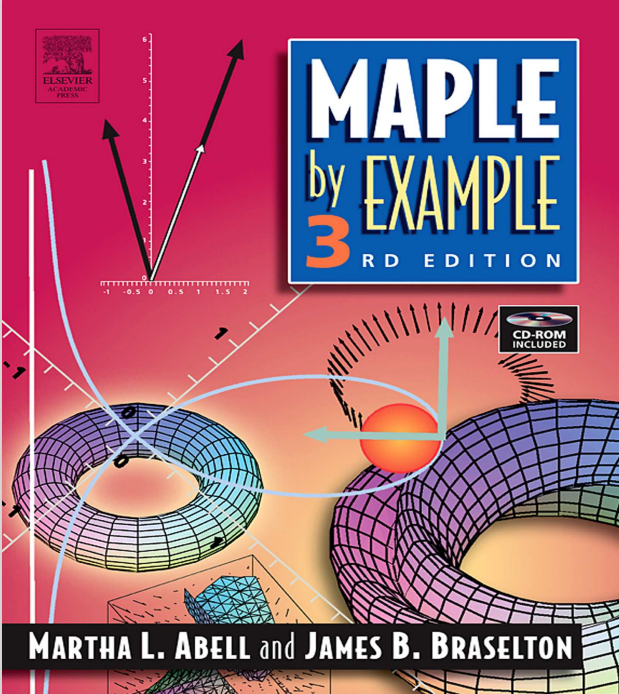
\includegraphics[height=7cm]{Mbe.PNG}
                \caption{Martha L. Abell,James B. Braselton, Maple by example, Third Edition, [M]. Acdemic Press, 2005}
                \label{Maple by example}
            \end{minipage}
        \end{figure}
        \autoref{fig:用 Maple 学大学数学} 是Maple入门级别的教材,强调Maple在微积分、
        线性代数以及数理统计方面的应用,适合第一次接触Maple的大学生。
        里面的讲解非常详细,例子稍显不足,可以用后面提到的参考书补充。

        \autoref{Maple by example} \cite[Maple by example]{abell2005maple} 是进阶级别的读物,给出了相当丰富而且精美
        的例子,十分值得推荐。比图1中的例子更加详
        实和丰富,也要更加专业,建议数学专业的同学读
        这本。

        \begin{figure}[htbp]
            \centering
            \begin{minipage}[t]
                {0.45\textwidth}
                \centering
                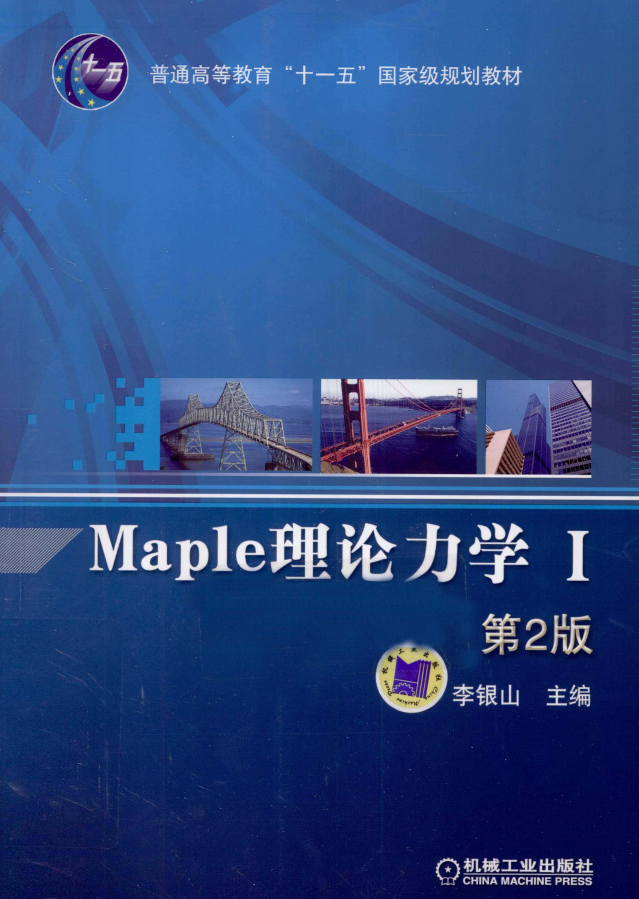
\includegraphics[height=7cm]{Maple TM.PNG}
                \caption{李银山.Maple理论力学I [M].2版.北京:机械工业出版社,2013.
                李银山.Maple理论力学II [M].2版.北京:机械工业出版社,2013.
                }

                \label{Maple理论力学I}
            \end{minipage}
            \quad
            \begin{minipage}[t]
                {0.45\textwidth}
                \centering
                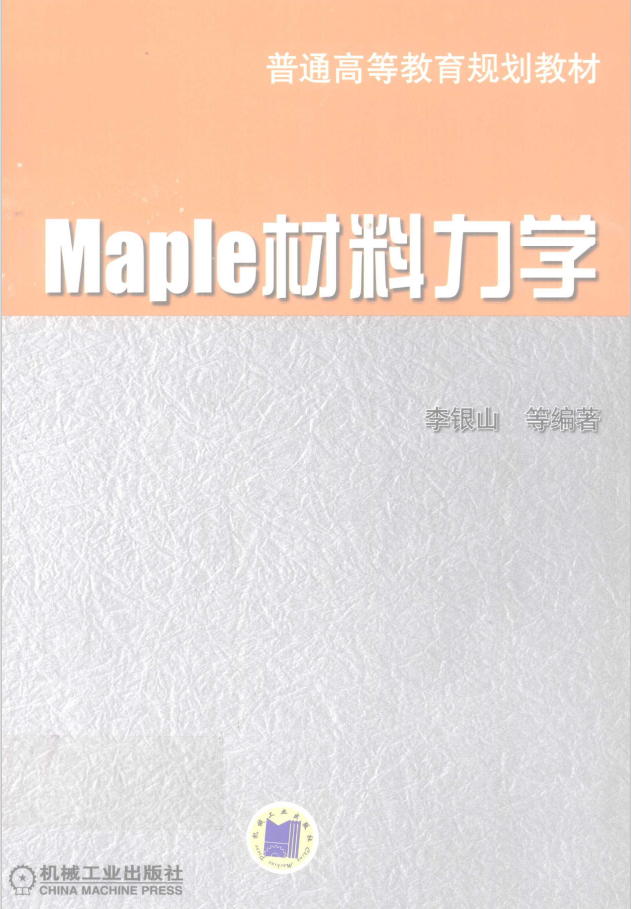
\includegraphics[height=7cm]{Maple MM.PNG}
                \caption{李银山.Maple材料力学 [M].北京:机械工业出版社,2013.}
                \label{Maple 材料力学}
            \end{minipage}

        \end{figure}
        \autoref{Maple理论力学I} \cite[Maple 理论力学 I]{李银山2013maple} 则更侧重Maple在力学、机械、土木等专业的理论力学计算方面的应用,
        给出的代码在最新版本的Maple中有的已经过时了,但是依旧不失为学
        习Maple和理论力学的好教材。

        \autoref{Maple 材料力学} \cite[Maple 材料力学]{李银山2013maple2} 是中规中矩的材料力学教材,提供了很多材料力学数值计算的经典方法,
        涉及到一些进阶应用。
    \end{spacing}
\end{large}


\restoregeometry